
\begin{center}
\begin{figure*}
\begin{tabular}{c}
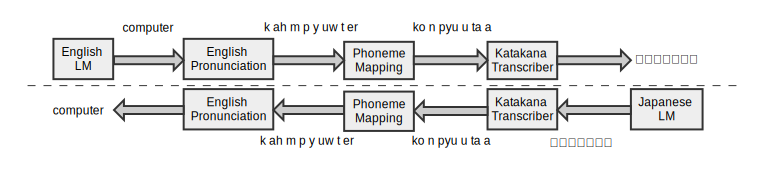
\includegraphics[scale=0.58]{figures/fsts}\tabularnewline
\end{tabular}
\caption{\label{font-table} The transliteration generative story as a cascade of FSTs . \textbf{Top:} transliteration of the word ``computer'' to Japanese. \textbf{Bottom:} the reverse process. Each box represents a transducer. In PAT for deciphering transliterations, the two cascades are jointly trained to maximize both the data log-likelihood and the parameter agreement of the two (shaded) phoneme mapping models.}
\label{fig:fsts}
\end{figure*}
\end{center}

\section{Transliteration}
In this section we show that PAT leads to better transliteration models even without parallel data.

\subsection{Generative Story}
Transliteration is a mapping of terms between writing systems of different languages. 
Usually, the transliterator tries to preserve the sound of a term as it is uttered in the original language. 
For example, the word ``computer'' in English is transliterated to Japanese as ``ko n pyu u ta a'' (in Romaji). 
The process that restores transliterated foreign words to their original script is called \emph{back-transliteration}.

Knight and Graehl \cite{KG98} suggest a generative story for transliteration of English into Japanese (see top of Figure \ref{fig:fsts}): 
\begin{enumerate}
\item First, a word $w$ is generated according to an English language model
$\PP(w)$.
\item $w$ is then mapped to a sequence of English phonemes $\mathbf{e}$ according to a pronunciation model.
\item The phoneme sequence $\mathbf{e}$ is mapped to a sequence of Japanese phonemes $\mathbf{j}$
according to a phoneme mapping model $\PP(\mathbf{j}\mid \mathbf{e})$.
\item Finally, the Japanese phoneme sequence $\mathbf{j}$ is mapped to a
Japanese word $k$ in Katakana.
\end{enumerate}

Knight and Graehl \cite{KG98} construct and train these FSTs independently.
In particular, the phoneme mapping model $\PP(\mathbf{j_{m}}| \mathbf{e_{m}})$ is trained over
a parallel phoneme corpus $\{(\mathbf{e_{n}},\, \mathbf{j_{n}})\}$.

\subsection{Deciphering Transliterations}
Collecting parallel data is often a time consuming and laborious process.
To combat the need for parallel data Ravi and Knight \cite{RK09} suggest learning to transliterate in the \emph{decipherment} setting:
In decipherment, only Japanese pronunciations $J=\{\mathbf{j_{n}}\}_{n=1}^{|J|}$ need be collected.
Treating the English pronunciation as missing data, a Japanese phoneme sequence $\mathbf{j}$ is viewed as being generated by all English pronunciations $\mathbf{e}$ producible by the language and pronunciation model:
$P(\mathbf{j}) = \sum_{\mathbf{e}}\PP(\mathbf{e})\cdot \PP(\mathbf{j}\mid \mathbf{e})$.
As a result, the data log-likelihood takes the form:
\begin{align}
L(J)& = \sum_{\mathbf{j}\in J} \log \sum_{\mathbf{e}} \PP(\mathbf{j}\mid \mathbf{e})\cdot \PP(\mathbf{e})
\end{align}
Once the model is trained, back-transliteration (decoding) of Japanese words back to English can be done using the Viterbi algorithm.

%We note a few points:
%\begin{itemize}
%\item The computational cost of solving this problem is much higher than the parallel case since we are forced to use the language and pronunciation models during training time. 
%\item Only the phoneme mapping parameters $P(j_{m}\mid e_{m})$ are trained while
%the other FSTs' parameters are kept fixed.
%\end{itemize}

\subsection{Parameter Agreement Training}
In PAT, the model corresponding to the inverse generative story is also used.
This inverse process is illustrated at the bottom of Figure \ref{fig:fsts}.

The training data for the reverse direction consists of set of English pronunciations  $E=\{\mathbf{e_n}\}_{n=1}^{|E|}$ and independent training maximizes:
\begin{align}
L(E)& = \sum_{\mathbf{e}\in E} \log \sum_{\mathbf{j}} \QQ(\mathbf{e}\mid \mathbf{j})\cdot \QQ(j)
\end{align}
To apply PAT, we maximize the joint regularized objective function:
\begin{align}
L(J) + L(E) + \lambda R(\PP(\mathbf{j}|\mathbf{e}), \QQ(\mathbf{e}|\mathbf{j}))
\label{eqn:dec_obj}
\end{align}
Once the two models are trained, Japanese words can be decoded using either model. 
In practice we followed Ravi and Knight and used the $\PP$.
\begin{figure*}[t]
\begin{center}
\begin{tabular}{ccc}
 &  & \tabularnewline
 & 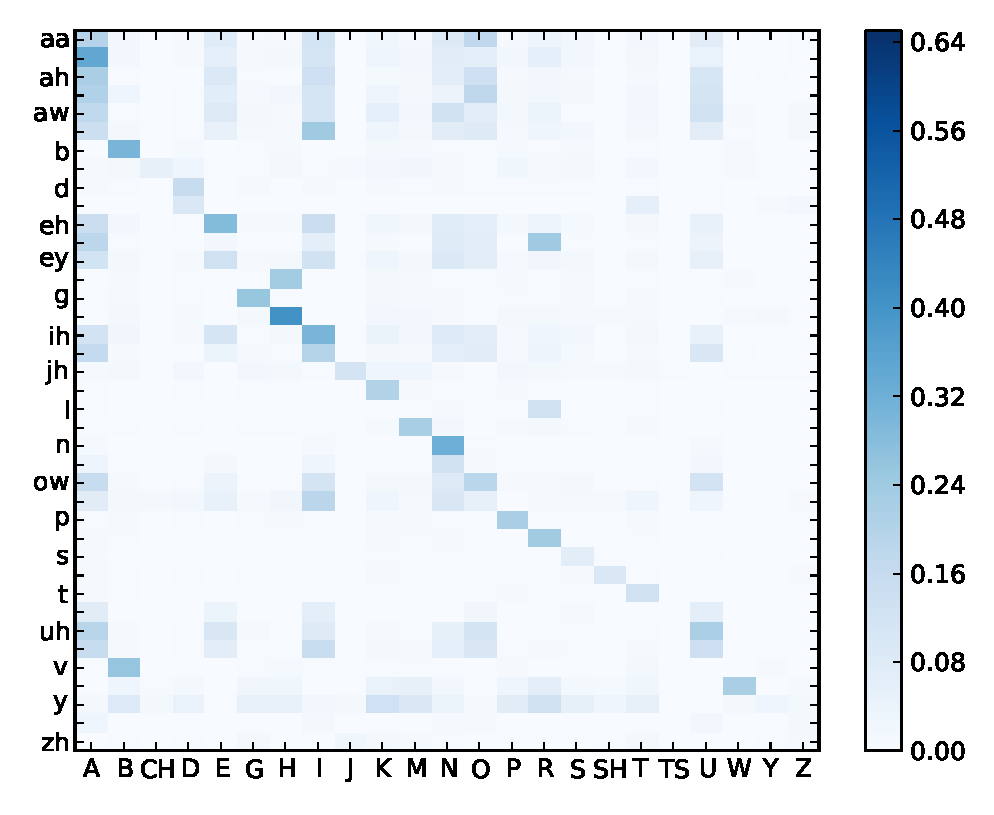
\includegraphics[scale=0.4]{figures/model_11_vanilla} &
 \includegraphics[scale=0.4]{figures/model_11_gm}\tabularnewline
 &  & \tabularnewline
\end{tabular}
\caption{Compared to independent training. PAT (right) learns sparser, peaked models.}
\label{fig:mapping}
\end{center}
\end{figure*}


\subsection{Decipherment Experiments}
Ravi and Knight \cite{RK09} compare back-transliteration whole-name error rates (WNER) on a list of 100 US senator names (In WNER, a decoding is correct if both the first and last name are decoded correctly).
They report 40\% error rate in the
parallel setting, and a 73\% error rate when using their best decipherment setting.

In order to compare PAT against independent training, we reproduced the decipherment setting \cite{RK09}.
For the FST machinery, we prepared:
\begin{itemize}
\item An English pronunciation FST from the CMU pronunciation dictionary. A Japanese pronunciation FST that was hand built.
\item Pronounceable word unigram LMs, constructed over the top ~40K most frequent capitalized words in the gigaword corpus and the top ~25K most frequent Katakana terms in the Japanese news 2005-2008 Leipzig corpora 
%(http://corpora.informatik.uni-leipzig.de/download.html)
\item for $\PP$, We implemented an FST similar to the best setting reported by \cite{RK09}. We note that $\PP$ is restricted to either 1-to-1 or 1-to-2 phoneme mappings. $\QQ$ was taken to be the reverse FST.
% (e.g., consonant parity. See details in the paper.)
\end{itemize}
For training data we take $E$ and $J$ to be the pronunciations of the top 50\% most frequent terms in their language models.
Using the entire set lead to poor baseline results, possibly since uncommon English terms do not get transliterated, and uncommon Japanese may be borrowed from a language other than English.
It note that $E$ and $J$ are far from being parallel, since they were collected over non parallel corpora.

In training time we maximized the objective (Equation \ref{eqn:dec_obj}) with respect to the phoneme mapping models $\PP, \QQ$ and over $\lambda\in\{1,2,3,4\}$. Training was stopped after 15 EM iterations.

The development set consistent of 50 frequent Japanese words and their English origin. 
We selected the NER minimizing model over the 15 iterations, $\lambda$ and a weight  $\alpha \in \{1,2,3\}$ that exponentiated the $\PP$ parameters before decoding. 

We compiled our own list of 100 US statesmen and used it as a test set. 
Table \ref{tbl:transliteration_results} reports WNER, average normalized edit distance  (NED) and the number of $\PP$ parameters with value greater than 0.01 ($\PP>0.01$) as an indication of model sparsity.

\begin{table}[h]
\begin{center}
\begin{tabular}{|c|c|c|c|}
\cline{2-4} 
\multicolumn{1}{c|}{} & WNER & NED & $\PP > 0.01$\tabularnewline
\hline 
Independent & 67\% & 23.18 & 649\tabularnewline
\hline 
PAT (our) & 59\% & 17.35 & 421\tabularnewline
\hline 
parallel data & 43\% & 10.8 & 152\tabularnewline
\hline 
\end{tabular}
\label{tbl:transliteration_results}
\caption{PAT reduces error rates and learns sparser models.}
\end{center}
\end{table}

Further evidence that PAT learns sparser models can be seen in Figure \ref{fig:mapping} which compares the 1-1 phoneme mapping of the selected $\PP$ decipherment models.


